\documentclass[11pt]{article}\usepackage[]{graphicx}\usepackage[]{color}
% maxwidth is the original width if it is less than linewidth
% otherwise use linewidth (to make sure the graphics do not exceed the margin)
\makeatletter
\def\maxwidth{ %
  \ifdim\Gin@nat@width>\linewidth
    \linewidth
  \else
    \Gin@nat@width
  \fi
}
\makeatother

\definecolor{fgcolor}{rgb}{0.345, 0.345, 0.345}
\newcommand{\hlnum}[1]{\textcolor[rgb]{0.686,0.059,0.569}{#1}}%
\newcommand{\hlstr}[1]{\textcolor[rgb]{0.192,0.494,0.8}{#1}}%
\newcommand{\hlcom}[1]{\textcolor[rgb]{0.678,0.584,0.686}{\textit{#1}}}%
\newcommand{\hlopt}[1]{\textcolor[rgb]{0,0,0}{#1}}%
\newcommand{\hlstd}[1]{\textcolor[rgb]{0.345,0.345,0.345}{#1}}%
\newcommand{\hlkwa}[1]{\textcolor[rgb]{0.161,0.373,0.58}{\textbf{#1}}}%
\newcommand{\hlkwb}[1]{\textcolor[rgb]{0.69,0.353,0.396}{#1}}%
\newcommand{\hlkwc}[1]{\textcolor[rgb]{0.333,0.667,0.333}{#1}}%
\newcommand{\hlkwd}[1]{\textcolor[rgb]{0.737,0.353,0.396}{\textbf{#1}}}%
\let\hlipl\hlkwb

\usepackage{framed}
\makeatletter
\newenvironment{kframe}{%
 \def\at@end@of@kframe{}%
 \ifinner\ifhmode%
  \def\at@end@of@kframe{\end{minipage}}%
  \begin{minipage}{\columnwidth}%
 \fi\fi%
 \def\FrameCommand##1{\hskip\@totalleftmargin \hskip-\fboxsep
 \colorbox{shadecolor}{##1}\hskip-\fboxsep
     % There is no \\@totalrightmargin, so:
     \hskip-\linewidth \hskip-\@totalleftmargin \hskip\columnwidth}%
 \MakeFramed {\advance\hsize-\width
   \@totalleftmargin\z@ \linewidth\hsize
   \@setminipage}}%
 {\par\unskip\endMakeFramed%
 \at@end@of@kframe}
\makeatother

\definecolor{shadecolor}{rgb}{.97, .97, .97}
\definecolor{messagecolor}{rgb}{0, 0, 0}
\definecolor{warningcolor}{rgb}{1, 0, 1}
\definecolor{errorcolor}{rgb}{1, 0, 0}
\newenvironment{knitrout}{}{} % an empty environment to be redefined in TeX

\usepackage{alltt}

\usepackage[top=25truemm,bottom=25truemm,left=25truemm,right=25truemm]{geometry}
\geometry{a4paper}

\usepackage{amsmath}
\usepackage{amssymb}
\usepackage{amsthm}
\usepackage{bm}
\usepackage{bbm}
\usepackage{mathtools}
\allowdisplaybreaks

\usepackage{graphicx}
\usepackage{float}
\usepackage{hyperref}
\usepackage{enumitem}
\usepackage{booktabs}

\DeclareMathOperator*{\plim}{plim}
\DeclareMathOperator*{\var}{var}
\DeclareMathOperator*{\cov}{cov}
\DeclareMathOperator*{\corr}{corr}

\newcommand{\indep}{\perp \!\!\! \perp}
\newcommand{\R}{\mathbb{R}}
\newcommand{\I}{\mathbbm{1}}
\newcommand{\argmax}{\mathop{\rm arg~max}\limits}
\newcommand{\argmin}{\mathop{\rm arg~min}\limits}

\title{Topics on R\\Example R Codes} 
\author{Konan Hara\footnote{Department of Economics, University of Arizona. E-mail: harakonan@email.arizona.edu}}
\date{September 8, 2021}
\IfFileExists{upquote.sty}{\usepackage{upquote}}{}
\begin{document}

\maketitle{}



\section{Getting Help}

\begin{knitrout}
\definecolor{shadecolor}{rgb}{0.969, 0.969, 0.969}\color{fgcolor}\begin{kframe}
\begin{alltt}
\hlkwd{help}\hlstd{(matrix)}
\hlkwd{example}\hlstd{(matrix)}
\end{alltt}
\begin{verbatim}
## 
## matrix> is.matrix(as.matrix(1:10))
## [1] TRUE
## 
## matrix> !is.matrix(warpbreaks)  # data.frame, NOT matrix!
## [1] TRUE
## 
## matrix> warpbreaks[1:10,]
##    breaks wool tension
## 1      26    A       L
## 2      30    A       L
## 3      54    A       L
## 4      25    A       L
## 5      70    A       L
## 6      52    A       L
## 7      51    A       L
## 8      26    A       L
## 9      67    A       L
## 10     18    A       M
## 
## matrix> as.matrix(warpbreaks[1:10,])  # using as.matrix.data.frame(.) method
##    breaks wool tension
## 1  "26"   "A"  "L"    
## 2  "30"   "A"  "L"    
## 3  "54"   "A"  "L"    
## 4  "25"   "A"  "L"    
## 5  "70"   "A"  "L"    
## 6  "52"   "A"  "L"    
## 7  "51"   "A"  "L"    
## 8  "26"   "A"  "L"    
## 9  "67"   "A"  "L"    
## 10 "18"   "A"  "M"    
## 
## matrix> ## Example of setting row and column names
## matrix> mdat <- matrix(c(1,2,3, 11,12,13), nrow = 2, ncol = 3, byrow = TRUE,
## matrix+                dimnames = list(c("row1", "row2"),
## matrix+                                c("C.1", "C.2", "C.3")))
## 
## matrix> mdat
##      C.1 C.2 C.3
## row1   1   2   3
## row2  11  12  13
\end{verbatim}
\begin{alltt}
\hlkwd{help.search}\hlstd{(}\hlstr{"linearmodels"}\hlstd{)}
\hlkwd{help}\hlstd{(}\hlkwc{package}\hlstd{=}\hlstr{"sandwich"}\hlstd{)}
\end{alltt}
\end{kframe}
\end{knitrout}

\section{R Objects}

\subsection{Numerics, Characters, Logicals, and Factors}

\begin{knitrout}
\definecolor{shadecolor}{rgb}{0.969, 0.969, 0.969}\color{fgcolor}\begin{kframe}
\begin{alltt}
\hlcom{# numeric}
\hlstd{n} \hlkwb{<-} \hlnum{100}
\hlkwd{class}\hlstd{(n)}
\end{alltt}
\begin{verbatim}
## [1] "numeric"
\end{verbatim}
\begin{alltt}
\hlcom{# numeric}
\hlstd{c} \hlkwb{<-} \hlstr{"Konan"}
\hlkwd{class}\hlstd{(c)}
\end{alltt}
\begin{verbatim}
## [1] "character"
\end{verbatim}
\begin{alltt}
\hlcom{# logical}
\hlkwd{class}\hlstd{(}\hlnum{TRUE}\hlstd{)}
\end{alltt}
\begin{verbatim}
## [1] "logical"
\end{verbatim}
\begin{alltt}
\hlkwd{class}\hlstd{(}\hlnum{FALSE}\hlstd{)}
\end{alltt}
\begin{verbatim}
## [1] "logical"
\end{verbatim}
\begin{alltt}
\hlkwd{class}\hlstd{(T)}
\end{alltt}
\begin{verbatim}
## [1] "logical"
\end{verbatim}
\begin{alltt}
\hlkwd{class}\hlstd{(F)}
\end{alltt}
\begin{verbatim}
## [1] "logical"
\end{verbatim}
\begin{alltt}
\hlkwd{as.numeric}\hlstd{(}\hlnum{TRUE}\hlstd{)}
\end{alltt}
\begin{verbatim}
## [1] 1
\end{verbatim}
\begin{alltt}
\hlkwd{as.numeric}\hlstd{(}\hlnum{FALSE}\hlstd{)}
\end{alltt}
\begin{verbatim}
## [1] 0
\end{verbatim}
\begin{alltt}
\hlcom{# factor}
\hlstd{sample_num} \hlkwb{<-} \hlkwd{rbinom}\hlstd{(}\hlnum{10}\hlstd{,}\hlnum{1}\hlstd{,}\hlnum{0.5}\hlstd{)}
\hlstd{sample_num}
\end{alltt}
\begin{verbatim}
##  [1] 0 1 1 0 0 0 0 0 1 1
\end{verbatim}
\begin{alltt}
\hlstd{sample_factor} \hlkwb{<-} \hlkwd{factor}\hlstd{(sample_num}
        \hlstd{,} \hlkwc{levels} \hlstd{=} \hlkwd{c}\hlstd{(}\hlnum{0}\hlstd{,}\hlnum{1}\hlstd{)}
        \hlstd{,} \hlkwc{labels} \hlstd{=} \hlkwd{c}\hlstd{(}\hlstr{"control"}\hlstd{,}\hlstr{"treatment"}\hlstd{))}
\hlstd{sample_factor}
\end{alltt}
\begin{verbatim}
##  [1] control   treatment treatment control   control   control   control  
##  [8] control   treatment treatment
## Levels: control treatment
\end{verbatim}
\begin{alltt}
\hlkwd{class}\hlstd{(sample_factor)}
\end{alltt}
\begin{verbatim}
## [1] "factor"
\end{verbatim}
\end{kframe}
\end{knitrout}

\subsection{Vectors}

\begin{knitrout}
\definecolor{shadecolor}{rgb}{0.969, 0.969, 0.969}\color{fgcolor}\begin{kframe}
\begin{alltt}
\hlcom{# define a vector}
\hlstd{v} \hlkwb{<-} \hlkwd{c}\hlstd{(}\hlkwd{seq}\hlstd{(}\hlkwc{from} \hlstd{=} \hlnum{1}\hlstd{,} \hlkwc{to} \hlstd{=} \hlnum{5}\hlstd{,} \hlkwc{by} \hlstd{=} \hlnum{1}\hlstd{))}
\hlstd{v}
\end{alltt}
\begin{verbatim}
## [1] 1 2 3 4 5
\end{verbatim}
\begin{alltt}
\hlkwd{class}\hlstd{(v)}
\end{alltt}
\begin{verbatim}
## [1] "numeric"
\end{verbatim}
\begin{alltt}
\hlcom{# recycle rule}
\hlkwd{c}\hlstd{(}\hlkwd{seq}\hlstd{(}\hlnum{1}\hlstd{,}\hlnum{3}\hlstd{))} \hlopt{+} \hlkwd{c}\hlstd{(}\hlkwd{seq}\hlstd{(}\hlnum{1}\hlstd{,}\hlnum{4}\hlstd{))}
\end{alltt}


{\ttfamily\noindent\color{warningcolor}{\#\# Warning in c(seq(1, 3)) + c(seq(1, 4)): longer object length is not a multiple of shorter object length}}\begin{verbatim}
## [1] 2 4 6 5
\end{verbatim}
\begin{alltt}
\hlkwd{c}\hlstd{(}\hlkwd{seq}\hlstd{(}\hlnum{1}\hlstd{,}\hlnum{2}\hlstd{))} \hlopt{+} \hlkwd{c}\hlstd{(}\hlkwd{seq}\hlstd{(}\hlnum{1}\hlstd{,}\hlnum{4}\hlstd{))}
\end{alltt}
\begin{verbatim}
## [1] 2 4 4 6
\end{verbatim}
\begin{alltt}
\hlcom{# operations are vectorized}
\hlstd{v} \hlkwb{<-} \hlnum{1}\hlopt{:}\hlnum{5}
\hlstd{v}
\end{alltt}
\begin{verbatim}
## [1] 1 2 3 4 5
\end{verbatim}
\begin{alltt}
\hlkwd{sqrt}\hlstd{(v)}
\end{alltt}
\begin{verbatim}
## [1] 1.000000 1.414214 1.732051 2.000000 2.236068
\end{verbatim}
\end{kframe}
\end{knitrout}

\subsection{Matrices}

\begin{knitrout}
\definecolor{shadecolor}{rgb}{0.969, 0.969, 0.969}\color{fgcolor}\begin{kframe}
\begin{alltt}
\hlcom{# define a matrix}
\hlstd{m} \hlkwb{<-} \hlkwd{matrix}\hlstd{(}\hlnum{1}\hlopt{:}\hlnum{4}\hlstd{,} \hlkwc{nrow} \hlstd{=} \hlnum{2}\hlstd{,} \hlkwc{ncol} \hlstd{=} \hlnum{2}\hlstd{)}
\hlstd{m}
\end{alltt}
\begin{verbatim}
##      [,1] [,2]
## [1,]    1    3
## [2,]    2    4
\end{verbatim}
\begin{alltt}
\hlkwd{class}\hlstd{(m)}
\end{alltt}
\begin{verbatim}
## [1] "matrix" "array"
\end{verbatim}
\begin{alltt}
\hlcom{# transpose}
\hlkwd{t}\hlstd{(m)}
\end{alltt}
\begin{verbatim}
##      [,1] [,2]
## [1,]    1    2
## [2,]    3    4
\end{verbatim}
\begin{alltt}
\hlcom{# dimension}
\hlkwd{dim}\hlstd{(m)}
\end{alltt}
\begin{verbatim}
## [1] 2 2
\end{verbatim}
\begin{alltt}
\hlcom{# length}
\hlkwd{length}\hlstd{(m)}
\end{alltt}
\begin{verbatim}
## [1] 4
\end{verbatim}
\begin{alltt}
\hlcom{# indexing}
\hlstd{m[}\hlnum{2}\hlstd{,}\hlnum{1}\hlstd{]}
\end{alltt}
\begin{verbatim}
## [1] 2
\end{verbatim}
\begin{alltt}
\hlstd{m[}\hlnum{2}\hlstd{,]}
\end{alltt}
\begin{verbatim}
## [1] 2 4
\end{verbatim}
\begin{alltt}
\hlstd{m[,}\hlnum{1}\hlstd{]}
\end{alltt}
\begin{verbatim}
## [1] 1 2
\end{verbatim}
\end{kframe}
\end{knitrout}

\subsection{Lists}

\begin{knitrout}
\definecolor{shadecolor}{rgb}{0.969, 0.969, 0.969}\color{fgcolor}\begin{kframe}
\begin{alltt}
\hlcom{# define a list}
\hlstd{l} \hlkwb{<-} \hlkwd{list}\hlstd{(v,m,}\hlkwd{c}\hlstd{(}\hlstr{"Tiemen"}\hlstd{,}\hlstr{"Konan"}\hlstd{))}
\hlstd{l}
\end{alltt}
\begin{verbatim}
## [[1]]
## [1] 1 2 3 4 5
## 
## [[2]]
##      [,1] [,2]
## [1,]    1    3
## [2,]    2    4
## 
## [[3]]
## [1] "Tiemen" "Konan"
\end{verbatim}
\begin{alltt}
\hlkwd{class}\hlstd{(l)}
\end{alltt}
\begin{verbatim}
## [1] "list"
\end{verbatim}
\begin{alltt}
\hlcom{# element-wise calculation}
\hlkwd{set.seed}\hlstd{(}\hlnum{100}\hlstd{)}
\hlstd{l} \hlkwb{<-} \hlkwd{list}\hlstd{(}\hlkwd{rnorm}\hlstd{(}\hlnum{2}\hlstd{),} \hlkwd{runif}\hlstd{(}\hlnum{4}\hlstd{),} \hlkwd{rgamma}\hlstd{(}\hlnum{6}\hlstd{,}\hlnum{1}\hlstd{,}\hlnum{1}\hlstd{))}
\hlstd{l}
\end{alltt}
\begin{verbatim}
## [[1]]
## [1] -0.5021924  0.1315312
## 
## [[2]]
## [1] 0.4685493 0.4837707 0.8124026 0.3703205
## 
## [[3]]
## [1] 0.5861317 0.7506868 0.1732320 0.8569455 0.2751689 0.5655790
\end{verbatim}
\begin{alltt}
\hlkwd{lapply}\hlstd{(l, mean)}
\end{alltt}
\begin{verbatim}
## [[1]]
## [1] -0.1853306
## 
## [[2]]
## [1] 0.5337608
## 
## [[3]]
## [1] 0.534624
\end{verbatim}
\end{kframe}
\end{knitrout}

\subsection{Data Frames}

\begin{knitrout}
\definecolor{shadecolor}{rgb}{0.969, 0.969, 0.969}\color{fgcolor}\begin{kframe}
\begin{alltt}
\hlcom{# define a data.frame}
\hlstd{df} \hlkwb{<-} \hlkwd{data.frame}\hlstd{(}
          \hlkwc{V1} \hlstd{=} \hlkwd{rep}\hlstd{(}\hlkwd{c}\hlstd{(}\hlnum{1}\hlstd{,} \hlnum{2}\hlstd{),} \hlnum{5}\hlstd{)[}\hlopt{-}\hlnum{10}\hlstd{]}
        \hlstd{,} \hlkwc{V2} \hlstd{=} \hlnum{1}\hlopt{:}\hlnum{9}
        \hlstd{,} \hlkwc{V3} \hlstd{=} \hlkwd{c}\hlstd{(}\hlnum{0.5}\hlstd{,} \hlnum{1.0}\hlstd{,} \hlnum{1.5}\hlstd{)}
        \hlstd{,} \hlkwc{V4} \hlstd{=} \hlkwd{rep}\hlstd{(LETTERS[}\hlnum{1}\hlopt{:}\hlnum{3}\hlstd{],} \hlnum{3}\hlstd{)}
        \hlstd{)}
\hlstd{df}
\end{alltt}
\begin{verbatim}
##   V1 V2  V3 V4
## 1  1  1 0.5  A
## 2  2  2 1.0  B
## 3  1  3 1.5  C
## 4  2  4 0.5  A
## 5  1  5 1.0  B
## 6  2  6 1.5  C
## 7  1  7 0.5  A
## 8  2  8 1.0  B
## 9  1  9 1.5  C
\end{verbatim}
\begin{alltt}
\hlcom{# define a data.table}
\hlcom{# install.packages("data.table")}
\hlkwd{library}\hlstd{(data.table)}
\hlstd{dt} \hlkwb{<-} \hlkwd{data.table}\hlstd{(}
          \hlkwc{V1} \hlstd{=} \hlkwd{rep}\hlstd{(}\hlkwd{c}\hlstd{(}\hlnum{1}\hlstd{,} \hlnum{2}\hlstd{),} \hlnum{5}\hlstd{)[}\hlopt{-}\hlnum{10}\hlstd{]}
        \hlstd{,} \hlkwc{V2} \hlstd{=} \hlnum{1}\hlopt{:}\hlnum{9}
        \hlstd{,} \hlkwc{V3} \hlstd{=} \hlkwd{c}\hlstd{(}\hlnum{0.5}\hlstd{,} \hlnum{1.0}\hlstd{,} \hlnum{1.5}\hlstd{)}
        \hlstd{,} \hlkwc{V4} \hlstd{=} \hlkwd{rep}\hlstd{(LETTERS[}\hlnum{1}\hlopt{:}\hlnum{3}\hlstd{],} \hlnum{3}\hlstd{)}
        \hlstd{)}
\hlstd{dt}
\end{alltt}
\begin{verbatim}
##    V1 V2  V3 V4
## 1:  1  1 0.5  A
## 2:  2  2 1.0  B
## 3:  1  3 1.5  C
## 4:  2  4 0.5  A
## 5:  1  5 1.0  B
## 6:  2  6 1.5  C
## 7:  1  7 0.5  A
## 8:  2  8 1.0  B
## 9:  1  9 1.5  C
\end{verbatim}
\begin{alltt}
\hlcom{# define a tibble}
\hlcom{# install.packages("dplyr")}
\hlcom{# dplyr is a part of the "tidyverse"}
\hlkwd{library}\hlstd{(dplyr)}
\end{alltt}


{\ttfamily\noindent\itshape\color{messagecolor}{\#\# \\\#\# Attaching package: 'dplyr'}}

{\ttfamily\noindent\itshape\color{messagecolor}{\#\# The following objects are masked from 'package:data.table':\\\#\# \\\#\#\ \ \ \  between, first, last}}

{\ttfamily\noindent\itshape\color{messagecolor}{\#\# The following objects are masked from 'package:stats':\\\#\# \\\#\#\ \ \ \  filter, lag}}

{\ttfamily\noindent\itshape\color{messagecolor}{\#\# The following objects are masked from 'package:base':\\\#\# \\\#\#\ \ \ \  intersect, setdiff, setequal, union}}\begin{alltt}
\hlcom{# V3 way doesn't work in tibble}
\hlstd{tib} \hlkwb{<-} \hlkwd{tibble}\hlstd{(}
          \hlkwc{V1} \hlstd{=} \hlkwd{rep}\hlstd{(}\hlkwd{c}\hlstd{(}\hlnum{1}\hlstd{,} \hlnum{2}\hlstd{),} \hlnum{5}\hlstd{)[}\hlopt{-}\hlnum{10}\hlstd{]}
        \hlstd{,} \hlkwc{V2} \hlstd{=} \hlnum{1}\hlopt{:}\hlnum{9}
        \hlstd{,} \hlkwc{V3} \hlstd{=} \hlkwd{c}\hlstd{(}\hlnum{0.5}\hlstd{,} \hlnum{1.0}\hlstd{,} \hlnum{1.5}\hlstd{)}
        \hlstd{,} \hlkwc{V4} \hlstd{=} \hlkwd{rep}\hlstd{(LETTERS[}\hlnum{1}\hlopt{:}\hlnum{3}\hlstd{],} \hlnum{3}\hlstd{)}
        \hlstd{)}
\end{alltt}


{\ttfamily\noindent\bfseries\color{errorcolor}{\#\# Error: Tibble columns must have compatible sizes.\\\#\# * Size 9: Existing data.\\\#\# * Size 3: Column `V3`.\\\#\# i Only values of size one are recycled.}}\begin{alltt}
\hlstd{tib} \hlkwb{<-} \hlkwd{tibble}\hlstd{(}
          \hlkwc{V1} \hlstd{=} \hlkwd{rep}\hlstd{(}\hlkwd{c}\hlstd{(}\hlnum{1}\hlstd{,} \hlnum{2}\hlstd{),} \hlnum{5}\hlstd{)[}\hlopt{-}\hlnum{10}\hlstd{]}
        \hlstd{,} \hlkwc{V2} \hlstd{=} \hlnum{1}\hlopt{:}\hlnum{9}
        \hlstd{,} \hlkwc{V3} \hlstd{=} \hlkwd{rep}\hlstd{(}\hlkwd{c}\hlstd{(}\hlnum{0.5}\hlstd{,} \hlnum{1.0}\hlstd{,} \hlnum{1.5}\hlstd{),} \hlnum{3}\hlstd{)}
        \hlstd{,} \hlkwc{V4} \hlstd{=} \hlkwd{rep}\hlstd{(LETTERS[}\hlnum{1}\hlopt{:}\hlnum{3}\hlstd{],} \hlnum{3}\hlstd{)}
        \hlstd{)}
\hlstd{tib}
\end{alltt}
\begin{verbatim}
## # A tibble: 9 x 4
##      V1    V2    V3 V4   
##   <dbl> <int> <dbl> <chr>
## 1     1     1   0.5 A    
## 2     2     2   1   B    
## 3     1     3   1.5 C    
## 4     2     4   0.5 A    
## 5     1     5   1   B    
## 6     2     6   1.5 C    
## 7     1     7   0.5 A    
## 8     2     8   1   B    
## 9     1     9   1.5 C
\end{verbatim}
\begin{alltt}
\hlcom{# demo using the R built-in iris data set}
\hlcom{# data.frame}
\hlkwd{head}\hlstd{(iris)}
\end{alltt}
\begin{verbatim}
##   Sepal.Length Sepal.Width Petal.Length Petal.Width Species
## 1          5.1         3.5          1.4         0.2  setosa
## 2          4.9         3.0          1.4         0.2  setosa
## 3          4.7         3.2          1.3         0.2  setosa
## 4          4.6         3.1          1.5         0.2  setosa
## 5          5.0         3.6          1.4         0.2  setosa
## 6          5.4         3.9          1.7         0.4  setosa
\end{verbatim}
\begin{alltt}
\hlcom{# data.table}
\hlstd{iris_dt} \hlkwb{<-} \hlkwd{as.data.table}\hlstd{(iris)}
\hlstd{iris_dt}
\end{alltt}
\begin{verbatim}
##      Sepal.Length Sepal.Width Petal.Length Petal.Width   Species
##   1:          5.1         3.5          1.4         0.2    setosa
##   2:          4.9         3.0          1.4         0.2    setosa
##   3:          4.7         3.2          1.3         0.2    setosa
##   4:          4.6         3.1          1.5         0.2    setosa
##   5:          5.0         3.6          1.4         0.2    setosa
##  ---                                                            
## 146:          6.7         3.0          5.2         2.3 virginica
## 147:          6.3         2.5          5.0         1.9 virginica
## 148:          6.5         3.0          5.2         2.0 virginica
## 149:          6.2         3.4          5.4         2.3 virginica
## 150:          5.9         3.0          5.1         1.8 virginica
\end{verbatim}
\begin{alltt}
\hlcom{# tibble}
\hlstd{iris_tib} \hlkwb{<-} \hlkwd{as_tibble}\hlstd{(iris)}
\hlstd{iris_tib}
\end{alltt}
\begin{verbatim}
## # A tibble: 150 x 5
##    Sepal.Length Sepal.Width Petal.Length Petal.Width Species
##           <dbl>       <dbl>        <dbl>       <dbl> <fct>  
##  1          5.1         3.5          1.4         0.2 setosa 
##  2          4.9         3            1.4         0.2 setosa 
##  3          4.7         3.2          1.3         0.2 setosa 
##  4          4.6         3.1          1.5         0.2 setosa 
##  5          5           3.6          1.4         0.2 setosa 
##  6          5.4         3.9          1.7         0.4 setosa 
##  7          4.6         3.4          1.4         0.3 setosa 
##  8          5           3.4          1.5         0.2 setosa 
##  9          4.4         2.9          1.4         0.2 setosa 
## 10          4.9         3.1          1.5         0.1 setosa 
## # ... with 140 more rows
\end{verbatim}
\begin{alltt}
\hlcom{# summary statistics}
\hlcom{# data.frame way}
\hlkwd{summary}\hlstd{(iris)}
\end{alltt}
\begin{verbatim}
##   Sepal.Length    Sepal.Width     Petal.Length    Petal.Width   
##  Min.   :4.300   Min.   :2.000   Min.   :1.000   Min.   :0.100  
##  1st Qu.:5.100   1st Qu.:2.800   1st Qu.:1.600   1st Qu.:0.300  
##  Median :5.800   Median :3.000   Median :4.350   Median :1.300  
##  Mean   :5.843   Mean   :3.057   Mean   :3.758   Mean   :1.199  
##  3rd Qu.:6.400   3rd Qu.:3.300   3rd Qu.:5.100   3rd Qu.:1.800  
##  Max.   :7.900   Max.   :4.400   Max.   :6.900   Max.   :2.500  
##        Species  
##  setosa    :50  
##  versicolor:50  
##  virginica :50  
##                 
##                 
## 
\end{verbatim}
\begin{alltt}
\hlcom{# data.table way}
\hlstd{iris_dt[,} \hlkwd{.}\hlstd{(}
          \hlkwc{count} \hlstd{= .N}
        \hlstd{,} \hlkwc{mean_sep} \hlstd{=} \hlkwd{mean}\hlstd{(Sepal.Length)}
        \hlstd{,} \hlkwc{mean_pet} \hlstd{=} \hlkwd{mean}\hlstd{(Petal.Length)}
        \hlstd{),} \hlkwc{by} \hlstd{=} \hlkwd{.}\hlstd{(Species)]}
\end{alltt}
\begin{verbatim}
##       Species count mean_sep mean_pet
## 1:     setosa    50    5.006    1.462
## 2: versicolor    50    5.936    4.260
## 3:  virginica    50    6.588    5.552
\end{verbatim}
\begin{alltt}
\hlcom{# tibble way}
\hlstd{iris_tib} \hlopt
        \hlkwd{group_by}\hlstd{(Species)} \hlopt
        \hlkwd{summarise}\hlstd{(}
                  \hlkwc{count} \hlstd{=} \hlkwd{n}\hlstd{()}
                \hlstd{,} \hlkwc{mean_sep} \hlstd{=} \hlkwd{mean}\hlstd{(Sepal.Length)}
                \hlstd{,} \hlkwc{mean_pet} \hlstd{=} \hlkwd{mean}\hlstd{(Petal.Length)}
                \hlstd{)}
\end{alltt}
\begin{verbatim}
## # A tibble: 3 x 4
##   Species    count mean_sep mean_pet
## * <fct>      <int>    <dbl>    <dbl>
## 1 setosa        50     5.01     1.46
## 2 versicolor    50     5.94     4.26
## 3 virginica     50     6.59     5.55
\end{verbatim}
\end{kframe}
\end{knitrout}

\section{Loops}

\begin{knitrout}
\definecolor{shadecolor}{rgb}{0.969, 0.969, 0.969}\color{fgcolor}\begin{kframe}
\begin{alltt}
\hlcom{# for loop}
\hlstd{x} \hlkwb{<-} \hlkwd{seq}\hlstd{(}\hlnum{3}\hlstd{,}\hlnum{7}\hlstd{,}\hlnum{2}\hlstd{)}
\hlkwa{for} \hlstd{(i} \hlkwa{in} \hlstd{x)\{}
        \hlkwd{print}\hlstd{(i}\hlopt{^}\hlnum{2}\hlstd{)}
\hlstd{\}}
\end{alltt}
\begin{verbatim}
## [1] 9
## [1] 25
## [1] 49
\end{verbatim}
\begin{alltt}
\hlcom{# while loop}
\hlstd{i} \hlkwb{<-} \hlnum{3}
\hlkwa{while}\hlstd{(i} \hlopt{<=} \hlnum{7}\hlstd{)\{}
        \hlkwd{print}\hlstd{(i}\hlopt{^}\hlnum{2}\hlstd{)}
        \hlstd{i} \hlkwb{<-} \hlstd{i}\hlopt{+}\hlnum{2}
\hlstd{\}}
\end{alltt}
\begin{verbatim}
## [1] 9
## [1] 25
## [1] 49
\end{verbatim}
\begin{alltt}
\hlcom{# repeat loop}
\hlstd{i} \hlkwb{<-} \hlnum{3}
\hlkwa{repeat}\hlstd{\{}
        \hlkwd{print}\hlstd{(i}\hlopt{^}\hlnum{2}\hlstd{)}
        \hlstd{i} \hlkwb{<-} \hlstd{i}\hlopt{+}\hlnum{2}
        \hlkwa{if}\hlstd{(i} \hlopt{>} \hlnum{7}\hlstd{)\{}
                \hlkwa{break}
        \hlstd{\}}
\hlstd{\}}
\end{alltt}
\begin{verbatim}
## [1] 9
## [1] 25
## [1] 49
\end{verbatim}
\end{kframe}
\end{knitrout}

\section{Regressions}

We replicate Keizer et al. (2008)'s dataset based on the following information:
\begin{itemize}
\item $N_{X=0} = N_{X=1} = 77$;
\item $\bar{Y}_{X=0} = 0.33$ and $\bar{Y}_{X=1} = 0.69$.
\end{itemize}

\begin{knitrout}
\definecolor{shadecolor}{rgb}{0.969, 0.969, 0.969}\color{fgcolor}\begin{kframe}
\begin{alltt}
\hlcom{# use Keizer et al. (2008)'s dataset}
\hlstd{keizer_data} \hlkwb{<-} \hlkwd{data.table}\hlstd{(}
          \hlkwc{x} \hlstd{=} \hlkwd{c}\hlstd{(}\hlkwd{rep}\hlstd{(}\hlnum{0}\hlstd{,}\hlnum{77}\hlstd{),} \hlkwd{rep}\hlstd{(}\hlnum{1}\hlstd{,}\hlnum{77}\hlstd{))}
        \hlstd{,} \hlkwc{y} \hlstd{=} \hlkwd{c}\hlstd{(}\hlkwd{rep}\hlstd{(}\hlnum{1}\hlstd{,}\hlnum{25}\hlstd{),} \hlkwd{rep}\hlstd{(}\hlnum{0}\hlstd{,}\hlnum{52}\hlstd{),} \hlkwd{rep}\hlstd{(}\hlnum{1}\hlstd{,}\hlnum{53}\hlstd{),} \hlkwd{rep}\hlstd{(}\hlnum{0}\hlstd{,}\hlnum{24}\hlstd{))}
        \hlstd{)}

\hlcom{# linear model}
\hlstd{keizer_lm} \hlkwb{<-} \hlkwd{lm}\hlstd{(}\hlkwc{formula} \hlstd{= y}\hlopt{~}\hlstd{x,} \hlkwc{data} \hlstd{= keizer_data)}

\hlcom{# summary}
\hlkwd{summary}\hlstd{(keizer_lm)}
\end{alltt}
\begin{verbatim}
## 
## Call:
## lm(formula = y ~ x, data = keizer_data)
## 
## Residuals:
##     Min      1Q  Median      3Q     Max 
## -0.6883 -0.3247  0.3117  0.3117  0.6753 
## 
## Coefficients:
##             Estimate Std. Error t value Pr(>|t|)    
## (Intercept)  0.32468    0.05342   6.078 9.42e-09 ***
## x            0.36364    0.07555   4.813 3.55e-06 ***
## ---
## Signif. codes:  0 '***' 0.001 '**' 0.01 '*' 0.05 '.' 0.1 ' ' 1
## 
## Residual standard error: 0.4688 on 152 degrees of freedom
## Multiple R-squared:  0.1323,	Adjusted R-squared:  0.1265 
## F-statistic: 23.17 on 1 and 152 DF,  p-value: 3.553e-06
\end{verbatim}
\begin{alltt}
\hlcom{# attributes}
\hlkwd{attributes}\hlstd{(keizer_lm)}
\end{alltt}
\begin{verbatim}
## $names
##  [1] "coefficients"  "residuals"     "effects"       "rank"         
##  [5] "fitted.values" "assign"        "qr"            "df.residual"  
##  [9] "xlevels"       "call"          "terms"         "model"        
## 
## $class
## [1] "lm"
\end{verbatim}
\begin{alltt}
\hlcom{# two ways to get coefficients}
\hlstd{keizer_lm}\hlopt{$}\hlstd{coefficients}
\end{alltt}
\begin{verbatim}
## (Intercept)           x 
##   0.3246753   0.3636364
\end{verbatim}
\begin{alltt}
\hlkwd{coefficients}\hlstd{(keizer_lm)}
\end{alltt}
\begin{verbatim}
## (Intercept)           x 
##   0.3246753   0.3636364
\end{verbatim}
\begin{alltt}
\hlcom{# heteroskedasticity robust standard errors}
\hlcom{# install.packages("sandwich")}
\hlkwd{library}\hlstd{(sandwich)}
\hlcom{# White's estimator}
\hlstd{keizer_lm_vcm} \hlkwb{<-} \hlkwd{vcovHC}\hlstd{(keizer_lm,} \hlkwc{type} \hlstd{=} \hlstr{"HC0"}\hlstd{)}
\hlkwd{sqrt}\hlstd{(}\hlkwd{diag}\hlstd{(keizer_lm_vcm))}
\end{alltt}
\begin{verbatim}
## (Intercept)           x 
##  0.05336243  0.07505842
\end{verbatim}
\begin{alltt}
\hlcom{# Long & Ervin (2000)}
\hlstd{keizer_lm_vcm} \hlkwb{<-} \hlkwd{vcovHC}\hlstd{(keizer_lm,} \hlkwc{type} \hlstd{=} \hlstr{"HC3"}\hlstd{)}
\hlkwd{sqrt}\hlstd{(}\hlkwd{diag}\hlstd{(keizer_lm_vcm))}
\end{alltt}
\begin{verbatim}
## (Intercept)           x 
##  0.05406457  0.07604603
\end{verbatim}
\begin{alltt}
\hlcom{# Logit model}
\hlstd{keizer_logit} \hlkwb{<-} \hlkwd{glm}\hlstd{(}
          \hlstd{y}\hlopt{~}\hlstd{x}
        \hlstd{,} \hlkwc{family} \hlstd{=} \hlkwd{binomial}\hlstd{(}\hlkwc{link} \hlstd{=} \hlstr{"logit"}\hlstd{)}
        \hlstd{,} \hlkwc{data} \hlstd{= keizer_data}
        \hlstd{)}

\hlcom{# summary}
\hlkwd{summary}\hlstd{(keizer_logit)}
\end{alltt}
\begin{verbatim}
## 
## Call:
## glm(formula = y ~ x, family = binomial(link = "logit"), data = keizer_data)
## 
## Deviance Residuals: 
##     Min       1Q   Median       3Q      Max  
## -1.5269  -0.8861   0.8643   0.8643   1.4999  
## 
## Coefficients:
##             Estimate Std. Error z value Pr(>|z|)    
## (Intercept)  -0.7324     0.2434  -3.009  0.00262 ** 
## x             1.5246     0.3461   4.405 1.06e-05 ***
## ---
## Signif. codes:  0 '***' 0.001 '**' 0.01 '*' 0.05 '.' 0.1 ' ' 1
## 
## (Dispersion parameter for binomial family taken to be 1)
## 
##     Null deviance: 213.46  on 153  degrees of freedom
## Residual deviance: 192.62  on 152  degrees of freedom
## AIC: 196.62
## 
## Number of Fisher Scoring iterations: 4
\end{verbatim}
\begin{alltt}
\hlcom{# attributes}
\hlkwd{attributes}\hlstd{(keizer_logit)}
\end{alltt}
\begin{verbatim}
## $names
##  [1] "coefficients"      "residuals"         "fitted.values"    
##  [4] "effects"           "R"                 "rank"             
##  [7] "qr"                "family"            "linear.predictors"
## [10] "deviance"          "aic"               "null.deviance"    
## [13] "iter"              "weights"           "prior.weights"    
## [16] "df.residual"       "df.null"           "y"                
## [19] "converged"         "boundary"          "model"            
## [22] "call"              "formula"           "terms"            
## [25] "data"              "offset"            "control"          
## [28] "method"            "contrasts"         "xlevels"          
## 
## $class
## [1] "glm" "lm"
\end{verbatim}
\end{kframe}
\end{knitrout}

\section{Plots}

\begin{knitrout}
\definecolor{shadecolor}{rgb}{0.969, 0.969, 0.969}\color{fgcolor}\begin{kframe}
\begin{alltt}
\hlcom{# example data}
\hlstd{N} \hlkwb{<-} \hlnum{1000}
\hlstd{data} \hlkwb{<-} \hlkwd{data.table}\hlstd{(}
          \hlkwc{u} \hlstd{=} \hlkwd{rnorm}\hlstd{(N)}
        \hlstd{,} \hlkwc{x} \hlstd{=} \hlkwd{rnorm}\hlstd{(N)}
        \hlstd{)}
\hlstd{data[, y} \hlkwb{:=} \hlnum{2.5}\hlopt{-}\hlnum{0.25}\hlopt{*}\hlstd{x}\hlopt{+}\hlstd{u]}

\hlcom{# base style}
\hlkwd{plot}\hlstd{(data}\hlopt{$}\hlstd{x,data}\hlopt{$}\hlstd{y)}
\hlkwd{abline}\hlstd{(}\hlkwd{lm}\hlstd{(y}\hlopt{~}\hlstd{x,} \hlkwc{data}\hlstd{=data))}
\end{alltt}
\end{kframe}
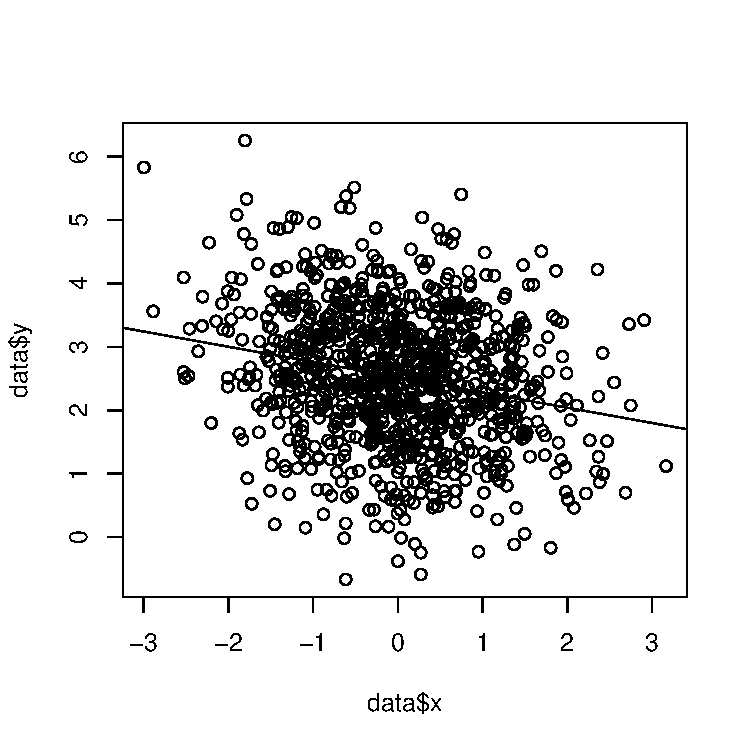
\includegraphics[width=\maxwidth]{figure/unnamed-chunk-9-1} 
\begin{kframe}\begin{alltt}
\hlcom{# ggplot style}
\hlcom{# install.packages("ggplot")}
\hlkwd{library}\hlstd{(ggplot2)}
\hlkwd{ggplot}\hlstd{(data,} \hlkwd{aes}\hlstd{(}\hlkwc{x}\hlstd{=x,} \hlkwc{y}\hlstd{=y))} \hlopt{+}
        \hlkwd{geom_point}\hlstd{()} \hlopt{+}
        \hlkwd{stat_smooth}\hlstd{(}\hlkwc{formula}\hlstd{=y}\hlopt{~}\hlstd{x,} \hlkwc{method}\hlstd{=lm)}
\end{alltt}
\end{kframe}
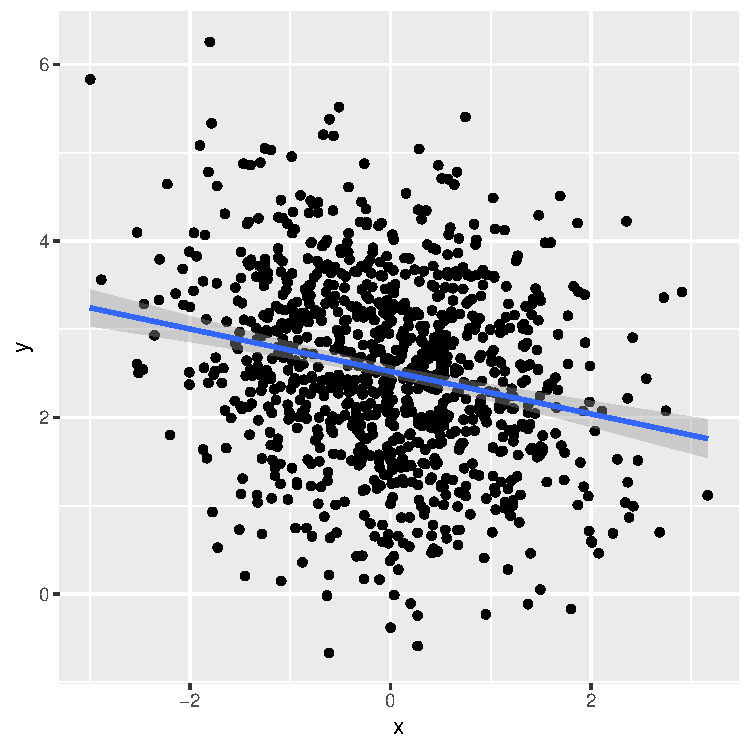
\includegraphics[width=\maxwidth]{figure/unnamed-chunk-9-2} 

\end{knitrout}

\section{User-defined Functions and Optimization}

We estimate the following model:
\begin{enumerate}
\item Data generating process is half $exp(0.5)$ and half $exp(0.75)$.
\item Our model is $y_i \text{ i.i.d.} \sim exp(\theta)$.
\item Estimate $\theta$ by MLE:
\begin{itemize}
\item Log-likelihood: $L(\theta; y_1,\dots,y_N) = N \log(\theta)-\theta \sum_{i=1}^N y_i $
\item Estimator for s.e.: $se(\theta) = \sqrt{\frac{\theta^2}{N}} $
\end{itemize}
\end{enumerate}

\begin{knitrout}
\definecolor{shadecolor}{rgb}{0.969, 0.969, 0.969}\color{fgcolor}\begin{kframe}
\begin{alltt}
\hlcom{# log-likelihood function}
\hlcom{# inputs}
\hlcom{# y: vector of samples}
\hlcom{# theta: parameter}
\hlstd{ll_func} \hlkwb{<-} \hlkwa{function}\hlstd{(}\hlkwc{y}\hlstd{,} \hlkwc{theta}\hlstd{)\{}
        \hlstd{N} \hlkwb{<-} \hlkwd{length}\hlstd{(y)}
        \hlstd{val} \hlkwb{<-} \hlstd{N}\hlopt{*}\hlkwd{log}\hlstd{(theta)}\hlopt{-}\hlstd{theta}\hlopt{*}\hlkwd{sum}\hlstd{(y)}
        \hlkwd{return}\hlstd{(val)}
\hlstd{\}}

\hlcom{# example data}
\hlstd{theta1} \hlkwb{<-} \hlnum{0.5}
\hlstd{theta2} \hlkwb{<-} \hlnum{0.75}
\hlstd{N} \hlkwb{<-} \hlnum{1000}
\hlstd{y1} \hlkwb{<-} \hlkwd{rexp}\hlstd{(}\hlnum{0.5}\hlopt{*}\hlstd{N,} \hlkwc{rate} \hlstd{= theta1)}
\hlstd{y2} \hlkwb{<-} \hlkwd{rexp}\hlstd{(}\hlnum{0.5}\hlopt{*}\hlstd{N,} \hlkwc{rate} \hlstd{= theta2)}
\hlstd{y} \hlkwb{<-} \hlkwd{c}\hlstd{(y1, y2)}

\hlcom{# optimization}
\hlstd{ll_op} \hlkwb{<-} \hlkwd{optimize}\hlstd{(}
          \hlstd{ll_func}
        \hlstd{,} \hlkwc{interval} \hlstd{=} \hlkwd{c}\hlstd{(}\hlnum{0.1}\hlstd{,}\hlnum{10}\hlstd{)}
        \hlstd{,} \hlkwc{y} \hlstd{= y}
        \hlstd{,} \hlkwc{maximum} \hlstd{=} \hlnum{TRUE}
        \hlstd{)}
\hlstd{ll_op}
\end{alltt}
\begin{verbatim}
## $maximum
## [1] 0.5789243
## 
## $objective
## [1] -1546.582
\end{verbatim}
\begin{alltt}
\hlcom{# estimate for theta}
\hlstd{theta_hat} \hlkwb{<-} \hlstd{ll_op}\hlopt{$}\hlstd{maximum}
\hlstd{theta_hat}
\end{alltt}
\begin{verbatim}
## [1] 0.5789243
\end{verbatim}
\begin{alltt}
\hlcom{# estimate for s.e.}
\hlkwd{sqrt}\hlstd{(theta_hat}\hlopt{^}\hlnum{2}\hlopt{/}\hlstd{N)}
\end{alltt}
\begin{verbatim}
## [1] 0.01830719
\end{verbatim}
\end{kframe}
\end{knitrout}

\end{document}





















